\chapter{Broken Symmetry, Goldstone Bosons, and Gauge Invariance}

We want to understand how a photon-like particle can acquire a mass. That is
the destination, but it is not a sensible starting point. A direct mass term
for a gauge field appears to destroy the very gauge invariance that makes the
theory consistent. Before we can see the escape route, we need two ideas in
working form:
\begin{enumerate}
  \item spontaneous symmetry breaking, especially for a continuous symmetry;
  \item gauge invariance, in which the symmetry operation may vary from one
        spacetime point to another.
\end{enumerate}
Neither idea can be replaced by a slogan. We shall build the first from a
magnet, translate it into scalar field theory, and discover the massless
Goldstone mode. We shall then take the same \(U(1)\) symmetry and make it
local, which forces us to introduce a vector potential and a covariant
derivative. Only at the end will the two threads be placed side by side. Their
actual union---the Higgs phenomenon---is the subject of the next lecture.

\section{A Symmetric Law with an Asymmetric Ground State}

\subsection{The two-state magnet}

Begin with a lattice of small magnets. Each spin can point up or down, and
neighboring spins lower their energy by pointing in the same direction. On a
three-dimensional cubic lattice a spin has six nearest neighbors, but the
precise coordination number is not important. What matters is the rule
\begin{equation}
  E_{\parallel}<E_{\rm antiparallel}.
\end{equation}
The microscopic rule is unchanged if every spin is reversed:
\begin{equation}
  \uparrow\longleftrightarrow\downarrow.
\end{equation}
Nevertheless, the lowest-energy configurations are not individually
symmetric. They are
\begin{equation}
  \{\uparrow\uparrow\uparrow\cdots\},
  \qquad
  \{\downarrow\downarrow\downarrow\cdots\}.
\end{equation}
The equations allow both, but a cold macroscopic sample must choose one.

This choice is extraordinarily sensitive. Fix one spin very far away to point
up. Its neighbors prefer to follow it, their neighbors prefer to follow them,
and the information propagates through the sample. A perturbation that is
arbitrarily small compared with the total system can select the orientation
of the whole ground state. That is the instability meant by
\emph{spontaneous} symmetry breaking.

\begin{classroomqa}
\audiencequestion{Can a neutral particle orient itself in a magnetic field?
\lecturetimestamp{00:05:14}}
\lecturerresponse{Yes. Electric neutrality does not imply the absence of a
magnetic moment. The neutron is neutral but has a magnetic moment because of
its internal charged constituents. A magnetic field can therefore distinguish
its spin orientations.}
\end{classroomqa}

\begin{classroomqa}
\audiencequestion{If the system changes orientation, does the change occur
everywhere at once? Can several reorientation waves coexist?
\lecturetimestamp{00:05:41--00:06:38}}
\lecturerresponse{The change propagates. One region tips its neighbors, rather
like a three-dimensional array of dominoes, and the disturbance travels as a
wave. Different regions can begin choosing independently, so several fronts
and several domains may be present before one orientation wins. We shall
return to precisely these waves when the symmetry becomes continuous.}
\end{classroomqa}

\subsection{Explicit breaking is a different theory}

Now place the sample in an external magnetic field pointing upward. An
isolated spin already has lower energy when it points up. The transformation
\(\uparrow\leftrightarrow\downarrow\) no longer leaves the energy unchanged:
the preference has been inserted into the law itself. This is \emph{explicit}
symmetry breaking.

The difference can be tested without knowing how the sample was prepared.
Take a very large specimen, hold its left boundary up, and hold its right
boundary down. If a bulk magnetic field explicitly favors up, the right-hand
constraint penetrates only a short distance. A macroscopic down region would
pay an energy proportional to its volume, so the bulk cannot remain divided
into two equally good phases.

Without the external bias, up and down have the same bulk energy. The
lowest-energy constrained state then contains an up domain, a down domain,
and a finite transition layer between them. The interface need not sit at the
geometrical center, but there is no volume pressure forcing one phase to
erase the other. This interface is a \emph{domain wall}, the characteristic
defect of this broken discrete symmetry.

\begin{figure}[htbp]
\centering
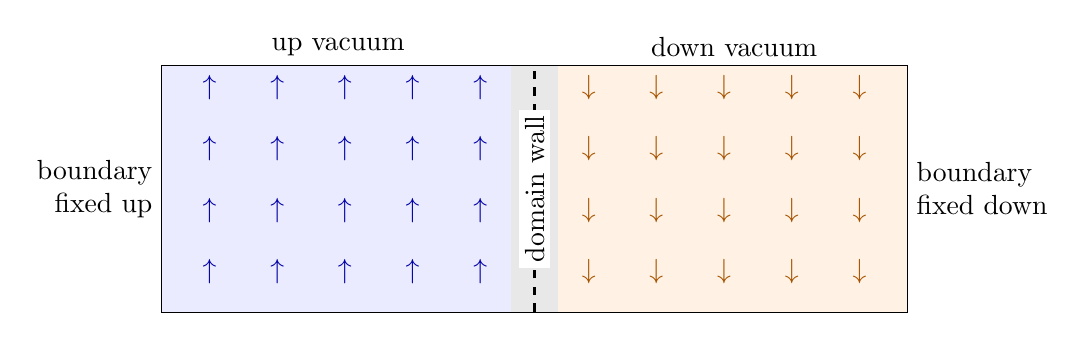
\begin{tikzpicture}[x=0.86cm,y=0.78cm]
  \draw[thick] (0,0) rectangle (11,4);
  \fill[blue!8] (0,0) rectangle (5.15,4);
  \fill[orange!10] (5.85,0) rectangle (11,4);
  \fill[gray!18] (5.15,0) rectangle (5.85,4);
  \foreach \x in {0.7,1.7,2.7,3.7,4.7}
    \foreach \y in {0.65,1.65,2.65,3.65}
      \node[blue!65!black] at (\x,\y) {$\uparrow$};
  \foreach \x in {6.3,7.3,8.3,9.3,10.3}
    \foreach \y in {0.65,1.65,2.65,3.65}
      \node[orange!65!black] at (\x,\y) {$\downarrow$};
  \draw[dashed,thick] (5.5,0) -- (5.5,4);
  \node[above] at (2.6,4) {up vacuum};
  \node[above] at (8.45,4) {down vacuum};
  \node[rotate=90,fill=white,inner sep=2pt] at (5.5,2) {domain wall};
  \node[left,align=right] at (0,2) {boundary\\fixed up};
  \node[right,align=left] at (11,2) {boundary\\fixed down};
\end{tikzpicture}
\caption{The boundary test for spontaneous breaking of a discrete symmetry.
Both bulk orientations have the same energy, so a wall can separate
macroscopic domains.}
\end{figure}

\begin{classroomqa}
\audiencequestion{Does the argument require interactions only between nearest
neighbors?\lecturetimestamp{00:18:18}}
\lecturerresponse{No. A second-neighbor interaction that also favors alignment
changes details but not the conclusion. More interesting behavior appears if
different ranges compete---nearest neighbors prefer alignment while
next-nearest neighbors prefer anti-alignment, for example. That produces
frustration and more complicated ordered phases, but it does not alter the
basic distinction being made here.}
\end{classroomqa}

\begin{classroomqa}
\audiencequestion{Does \emph{spontaneous} refer to the large derivative inside
the wall?\lecturetimestamp{00:19:05}}
\lecturerresponse{No. It refers to the fact that the underlying energy has no
up--down preference while the selected ground state does. The dramatic
response to an arbitrarily small perturbation reveals an instability. The
gradient merely tells us how much the interface costs.}
\end{classroomqa}

\begin{classroomqa}
\audiencequestion{Was the material already in one of the two states, or was
its state initially unknown?\lecturetimestamp{00:19:40}}
\lecturerresponse{That depends on its history. At high temperature thermal
motion can leave up and down spins mixed with nearly zero average
magnetization. As the material cools, patches choose different orientations,
domain walls form, and the domains coarsen. Chance and tiny environmental
perturbations determine which vacuum finally occupies most of the sample.}
\end{classroomqa}

\section{The Same Argument as Scalar Field Theory}

Replace the spins by a real scalar field \(\phi(\bm{x},t)\). With metric and
normalization conventions fixed once and for all, write
\begin{equation}
  \mathcal L
  =\frac12\,\partial_\mu\phi\,\partial^\mu\phi-V(\phi),
  \qquad
  \mathcal E
  =\frac12\dot\phi^{\,2}+\frac12(\nabla\phi)^2+V(\phi).
  \label{eq:l07-real-scalar}
\end{equation}
The relativistic shorthand in \(\mathcal L\) contains the positive
time-derivative term and negative spatial-gradient term; the Hamiltonian
energy density has both contributions positive.

Choose an even potential with two degenerate minima,
\begin{equation}
  V(\phi)=\frac{\lambda}{4}\left(\phi^2-f^2\right)^2,
  \qquad \lambda>0.
  \label{eq:l07-double-well}
\end{equation}
The Lagrangian is invariant under \(\phi\mapsto-\phi\), while either uniform
vacuum
\begin{equation}
  \phi(\bm{x})=+f,
  \qquad\hbox{or}\qquad
  \phi(\bm{x})=-f
\end{equation}
chooses one side. A potential with a unique minimum at \(\phi=0\), by
contrast, has a symmetric vacuum and is not spontaneously broken.

Fix \(\phi=+f\) on one side of a sample and \(\phi=-f\) on the other. The
field cannot jump without cost, because
\begin{equation}
  E_{\rm wall}
  =\int dx\left[
      \frac12\left(\frac{d\phi}{dx}\right)^2+V(\phi)-V(f)
    \right].
  \label{eq:l07-wall-energy}
\end{equation}
An abrupt jump makes \(d\phi/dx\) enormous. The minimum-energy wall therefore
spreads the change over a finite width, balancing gradient energy against the
potential cost of passing between the minima. The familiar kink solution for
the potential in Eq.~\eqref{eq:l07-double-well} is
\begin{equation}
  \phi_{\rm wall}(x)
  =f\tanh\!\left[f\sqrt{\frac{\lambda}{2}}\,(x-x_0)\right],
  \label{eq:l07-kink}
\end{equation}
an explicit realization of the smooth transition described at the board.
\editorialnote{The lecture argues from the shape of the potential and the
gradient term but does not solve the field equation. Equation
\eqref{eq:l07-kink} is included as the standard solution of that stated
model, making the qualitative wall concrete without changing the argument.}

Tilt the double well slightly and one minimum becomes lower. The Lagrangian
itself is then asymmetric. A wall can still appear temporarily, but the
higher-energy or false vacuum exerts a pressure on it; the wall moves and
the favored phase expands. This is the field-theory version of explicit
breaking by an external magnetic field.

So far the symmetry has been discrete. Particle physics is dominated by
continuous groups such as \(U(1)\), \(SU(2)\), and \(SU(3)\). A continuous
symmetry changes the defect story and introduces a new kind of particle.

\section{A Complex Field and Global \texorpdfstring{\(U(1)\)}{U(1)}}

\subsection{Rotations in an internal plane}

Let
\begin{equation}
  \phi=\phi_R+i\phi_I,
  \qquad
  \phi^*=\phi_R-i\phi_I,
  \qquad
  \phi^*\phi=\phi_R^2+\phi_I^2.
  \label{eq:l07-components}
\end{equation}
The \(\phi_R\) and \(\phi_I\) axes form an internal field space, not two
directions in ordinary space. A complex scalar is simply two real scalar
fields packaged so that rotations in this internal plane are manifest.

\begin{figure}[htbp]
\centering

\includegraphics[width=0.80\textwidth]{lecture_07_figure_02.png}
\caption{The complex field on the internal \((\phi_R,\phi_I)\)-plane. The
board records the decomposition of \(\phi\) and \(\phi^*\) and the invariant
radius \(\phi^*\phi\).}
\lectureframe{00:33:33}
\end{figure}

Use the Lagrangian
\begin{equation}
  \mathcal L
  =\partial_\mu\phi^*\,\partial^\mu\phi
   -V(\phi^*\phi).
  \label{eq:l07-complex-lagrangian}
\end{equation}
For a complex field the conventional factor \(1/2\) is absent, because this
single product already contains the kinetic terms of both real components.
The transformation
\begin{equation}
  \phi'(x)=e^{i\theta}\phi(x),
  \qquad
  \phi^{*\prime}(x)=e^{-i\theta}\phi^*(x)
  \label{eq:l07-global-u1}
\end{equation}
rotates every field value through the same angle. Here \(\theta\) is constant
in space and time. The prime labels the transformed field; it is not a
derivative.

Because \(\theta\) is constant,
\begin{equation}
  \partial_\mu\phi'=e^{i\theta}\partial_\mu\phi,
  \qquad
  \partial_\mu\phi^{*\prime}
  =e^{-i\theta}\partial_\mu\phi^*.
\end{equation}
The phases cancel in the kinetic term, and
\(\phi^{*\prime}\phi'=\phi^*\phi\). Thus every potential that depends only on
\(\phi^*\phi\) has the same symmetry. A term depending on \(\phi_R\) alone
would pick a direction in the internal plane and break it explicitly.

\subsection{A point minimum and a circle of minima}

There are two qualitatively different symmetric potentials. The first has
its only minimum at the origin, for example
\begin{equation}
  V_{\rm unbroken}=m^2\phi^*\phi,
  \qquad m^2>0.
\end{equation}
Its graph is a rotationally symmetric paraboloid. The vacuum \(\phi=0\)
stays fixed under every rotation, so the symmetry is unbroken.

Now choose
\begin{equation}
  V_{\rm broken}
  =-a\,\phi^*\phi+b(\phi^*\phi)^2,
  \qquad a,b>0.
  \label{eq:l07-mexican-hat}
\end{equation}
The negative quadratic term drives the field away from the origin, while the
positive quartic term prevents it from running to infinity. Writing
\(r^2=\phi^*\phi\), minimization gives
\begin{equation}
  \frac{dV}{d(r^2)}=-a+2br^2=0,
  \qquad
  r^2=f^2=\frac{a}{2b}.
  \label{eq:l07-vacuum-radius}
\end{equation}
The minima therefore form a circle. The potential is perfectly rotationally
symmetric, yet a uniform ground state must choose one point on that circle.

\begin{figure}[htbp]
\centering

\includegraphics[width=0.72\textwidth]{lecture_07_figure_06.png}
\caption{The symmetry-breaking potential drawn as a surface of revolution.
The origin is unstable and the degenerate minima form the circular trough.}
\lectureframe{00:37:25}
\end{figure}

Think of the field as a little arrow in this internal plane at every point of
ordinary space. The potential asks every arrow to have length \(f\). The
gradient energy asks nearby arrows to point in nearly the same direction.
The ground state consequently has the same angle everywhere, but no angle is
preferred by the law. That is continuous spontaneous symmetry breaking.

\section{From a Domain Wall to a Smooth Twist}

Repeat the boundary experiment. At the left boundary fix the field at a
vacuum point \(A\); at the right fix it at another vacuum point \(B\). A
localized jump would make the gradient large. Unlike the discrete case,
however, the field can remain at the bottom of the potential while changing
continuously around the circle.

At low energy write the field as \(\phi=f e^{i\alpha(x)}\). In one spatial
dimension the relevant energy is
\begin{equation}
  E[\alpha]
  =f^2\int_0^L dx\,\left(\frac{d\alpha}{dx}\right)^2.
  \label{eq:l07-angle-functional}
\end{equation}
For fixed endpoint angles, variation gives
\begin{equation}
  \frac{d^2\alpha}{dx^2}=0,
  \qquad
  \alpha(x)=\alpha_A+
    \frac{\alpha_B-\alpha_A}{L}\,x.
  \label{eq:l07-linear-twist}
\end{equation}
The preferred configuration spreads the twist uniformly through the sample.
Its energy scales as
\begin{equation}
  E_{\rm twist}
  =f^2\frac{(\alpha_B-\alpha_A)^2}{L},
  \label{eq:l07-twist-energy}
\end{equation}
so it can be made arbitrarily cheap by increasing \(L\).

\begin{figure}[htbp]
\centering
\begin{tikzpicture}[x=0.95cm,y=0.95cm]
  \begin{scope}
    \draw[->] (0,0) -- (6.2,0) node[right] {$x$};
    \draw[->] (0,0) -- (0,3.5) node[above] {$\alpha(x)$};
    \draw[very thick,blue!70!black] (0.45,0.65) -- (5.7,2.85);
    \fill (0.45,0.65) circle (1.8pt) node[left] {$\alpha_A$};
    \fill (5.7,2.85) circle (1.8pt) node[right] {$\alpha_B$};
    \node at (3.1,-0.65) {physical space};
  \end{scope}
  \begin{scope}[xshift=9.2cm,yshift=1.65cm]
    \draw[thick] (0,0) circle (1.8);
    \fill (1.55,-0.92) circle (1.8pt) node[below right] {$A$};
    \fill (-0.45,1.74) circle (1.8pt) node[above] {$B$};
    \draw[very thick,blue!70!black,-{Latex[length=2.5mm]}]
      (1.55,-0.92) arc[start angle=-31,end angle=104,radius=1.8];
    \node at (0,-2.35) {vacuum circle};
  \end{scope}
\end{tikzpicture}
\caption{The same low-energy configuration in two descriptions. The angle
varies linearly across physical space while the field follows the short arc
of the vacuum circle in internal space.}
\end{figure}

\begin{classroomqa}
\audiencequestion{There can be two ways around the circle. Which path does the
field take, and can it become trapped on the longer one?
\lecturetimestamp{00:41:54}}
\lecturerresponse{For generic endpoints the shorter angular route has the
smaller gradient and therefore the lower energy. Diametrically opposite
endpoints make the two simplest routes degenerate. A configuration prepared
by slowly moving an endpoint may retain an extra winding and become trapped
behind an energy barrier, but for a specified pair of ordinary endpoints the
untwisted shortest route is the ground state.}
\end{classroomqa}

\begin{classroomqa}
\audiencequestion{Could a path leave the bottom of the trough and cut across
the interior, becoming shorter overall?\lecturetimestamp{00:43:32}}
\lecturerresponse{In the low-energy, long-sample regime it does not pay to
climb the radial potential. Keeping the radius at its vacuum value and
varying the angle linearly minimizes the effective energy, as the
calculus-of-variations calculation above shows. For a finite system with a
specific potential one can minimize radial and angular motion together, but
the Goldstone conclusion concerns the arbitrarily long-wavelength limit in
which the smooth motion along the trough wins.}
\end{classroomqa}

\begin{classroomqa}
\audiencequestion{What changes if the circular trough is tilted so that one
angle is lower?\lecturetimestamp{00:44:33}}
\lecturerresponse{Then the symmetry is explicitly broken. One point becomes
the true ground state, motion along the circle acquires a restoring force,
and the angular excitation is no longer exactly massless.}
\end{classroomqa}

\section{Mass as the Cost of a Zero-Momentum Oscillation}

The smooth twist reveals a field whose energy comes only from gradients. To
understand why that means a massless particle, compare the relativistic
dispersion relation
\begin{equation}
  \omega^2=\bm{k}^2+m^2.
  \label{eq:l07-dispersion}
\end{equation}
A wave \(e^{i(\bm{k}\cdot\bm{x}-\omega t)}\) carries momentum \(\bm{k}\).
If \(m=0\), its energy tends to zero as the wavelength tends to infinity:
\(\omega=|\bm{k}|\to0\). If \(m\ne0\), a spatially homogeneous mode
\(\bm{k}=0\) still oscillates with frequency \(\omega=m\). The mass is the
irreducible zero-momentum energy.

This same distinction is visible in the Lagrangian. A term
\begin{equation}
  -\frac12m^2\varphi^2
\end{equation}
supplies a restoring force even for a homogeneous displacement. A field with
only derivative terms has no such restoring force: make its wavelength
longer, and its gradient energy approaches zero.

\subsection{Polar variables separate the two modes}

Write the broken complex field as
\begin{equation}
  \phi(x)=\rho(x)e^{i\alpha(x)}.
  \label{eq:l07-polar}
\end{equation}
Both \(\rho\) and \(\alpha\) are fields. Differentiation gives
\begin{align}
  \partial_\mu\phi
  &=e^{i\alpha}
    \left(\partial_\mu\rho+i\rho\,\partial_\mu\alpha\right),\\
  \partial_\mu\phi^*
  &=e^{-i\alpha}
    \left(\partial_\mu\rho-i\rho\,\partial_\mu\alpha\right).
\end{align}
The cross terms cancel, leaving
\begin{equation}
  \partial_\mu\phi^*\,\partial^\mu\phi
  =(\partial_\mu\rho)(\partial^\mu\rho)
   +\rho^2(\partial_\mu\alpha)(\partial^\mu\alpha).
  \label{eq:l07-polar-kinetic}
\end{equation}
Since \(\phi^*\phi=\rho^2\),
\begin{equation}
  \mathcal L
  =(\partial\rho)^2+\rho^2(\partial\alpha)^2-V(\rho^2).
  \label{eq:l07-polar-lagrangian}
\end{equation}
The potential contains \(\rho\) but not \(\alpha\). That absence is the
symmetry in its most useful form.

\begin{figure}[htbp]
\centering

\includegraphics[width=0.88\textwidth]{lecture_07_figure_03.png}
\caption{The polar-field Lagrangian, its boxed low-energy angular term, and
the symmetry-breaking potential. Radial motion climbs the potential; angular
motion follows the trough.}
\lectureframe{00:56:40}
\end{figure}

For a very low-energy excitation the field remains close to
\(\rho=f\). Then
\begin{equation}
  \mathcal L_{\rm angular}
  \simeq f^2(\partial_\mu\alpha)(\partial^\mu\alpha).
\end{equation}
Define the canonically normalized angular field, up to the convention used
for factors of \(1/2\), by
\begin{equation}
  \beta=\sqrt{2}\,f\alpha,
  \qquad
  \mathcal L_{\rm angular}
  =\frac12(\partial_\mu\beta)(\partial^\mu\beta).
  \label{eq:l07-goldstone-field}
\end{equation}
There is no \(\beta^2\) term. The quanta of this angular field are massless.
They are the Goldstone bosons.

The radial field behaves differently. Displace \(\rho\) from \(f\) everywhere
at once and it rolls back, overshoots, and oscillates about the trough. If
\(\rho=f+h\), expansion of Eq.~\eqref{eq:l07-mexican-hat} produces
\begin{equation}
  V(f+h)=V(f)+\frac12m_h^2h^2+\cdots,
\end{equation}
so \(h\) is massive. Geometrically, the angular direction is flat and the
radial direction is curved.

\begin{classroomqa}
\audiencequestion{If the field is displaced radially, does it simply drop
back down, and what happens next?\lecturetimestamp{00:57:10}}
\lecturerresponse{With no angular motion it falls toward the minimum,
overshoots, and oscillates radially. A homogeneous oscillation has zero
spatial momentum but nonzero frequency; that frequency is the mass of the
radial excitation. A homogeneous angular displacement, in contrast, lands on
another vacuum and has no restoring force.}
\end{classroomqa}

This is the content of the Goldstone principle in the present example:
spontaneously breaking a continuous global symmetry produces a massless mode
for each independent flat direction of the vacuum manifold.
\editorialnote{The statement assumes the usual conditions of relativistic
field theory. In nonrelativistic many-body systems the counting and
dispersion of Nambu--Goldstone modes can be subtler, but the lecture's
long-wavelength conclusion remains the right one for this relativistic
\(U(1)\) model.}

\section{Spin Waves, Strings, and Sound}

The theorem is abstract, but its mechanism is familiar. In an isotropic
ferromagnet all spins may be rotated together without changing the energy.
Let the orientation vary very slowly across the sample and one obtains a
spin wave. Its cost vanishes with its wave number, so it is the Goldstone
mode of broken spin-rotation symmetry.

A long elastic string supplies another picture. Ignore gravity and mount the
ends so that the whole string may be translated vertically. A uniform
vertical translation costs no energy. Let the translation vary slowly along
the string and it becomes a long-wavelength transverse wave. The uniform
symmetry operation has been promoted to a gentle position-dependent
deformation.

\begin{figure}[htbp]
\centering

\includegraphics[width=0.68\textwidth]{lecture_07_figure_04.png}
\caption{The slowly varying string profile drawn during the Goldstone-mode
analogy. The physical point is the small slope of a long-wavelength
deformation, not the vertical placement of the curve.}
\lectureframe{01:04:19}
\end{figure}

\begin{classroomqa}
\audiencequestion{Can the string carry oscillation energy while having zero
momentum?\lecturetimestamp{01:04:41}}
\lecturerresponse{One must distinguish vertical mechanical momentum from
wave momentum along the string. A standing wave can have zero net momentum
because it is a superposition of modes with \(+k\) and \(-k\), while still
carrying energy. In the field-theory analogy, momentum refers to the wave
number along the axis; the vertical displacement stands for the internal
field coordinate.}
\end{classroomqa}

A slinky gives the longitudinal version. Translate the entire idealized
infinite slinky along its axis and nothing changes. Translate neighboring
parts by slightly different amounts and the result is a gentle compression
wave. In a solid or fluid, long-wavelength sound similarly arises from
collective displacements and density variations. Spin waves, transverse
string waves, and sound are not the same microscopic excitation, but they
share the decisive pattern: a uniform continuous operation costs no energy,
and its slowly varying version becomes a soft mode.
\editorialnote{In a crystal, acoustic phonons are conventionally described as
Nambu--Goldstone modes of spontaneously broken continuous translations. The
string and slinky are mechanical analogies used in the lecture to expose the
same derivative-only energy structure.}

The terminology matters enough for a brief classroom joke: these are
\emph{Goldstone} bosons, named for Jeffrey Goldstone, not gauge bosons.
The lecture notes that Goldstone was a friend of Susskind's and then pivots
to the genuinely different subject of gauge invariance.

\section{From Global Phase Symmetry to Gauge Symmetry}

The \(U(1)\) phase symmetry has already appeared in the course as the symmetry
associated with conservation of charge. Charged particle fields are complex,
and multiplying such a field by a common phase leaves the global theory
unchanged. The word electric may be used for intuition, though the charge
could represent another \(U(1)\) quantum number. The real photon is massless;
the eventual target is a photon-like field such as the massive \(Z\).

The new question is whether
\begin{equation}
  \phi'(x)=e^{i\theta(x)}\phi(x)
  \label{eq:l07-local-u1}
\end{equation}
can be a symmetry when \(\theta\) varies arbitrarily through spacetime.
The function \(\theta(x)\) is a transformation parameter, not an additional
dynamical field. We test the proposal by differentiating:
\begin{equation}
  \partial_\mu\phi'
  =e^{i\theta}
   \left[\partial_\mu\phi+i(\partial_\mu\theta)\phi\right].
  \label{eq:l07-local-derivative}
\end{equation}
The extra term was absent for constant \(\theta\). For the conjugate,
\begin{equation}
  \partial_\mu\phi^{*\prime}
  =e^{-i\theta}
   \left[\partial_\mu\phi^*-i(\partial_\mu\theta)\phi^*\right].
\end{equation}
Their product is
\begin{align}
  \partial_\mu\phi^{*\prime}\partial^\mu\phi'
  ={}&
  \partial_\mu\phi^*\partial^\mu\phi
  i\left(
      \phi\,\partial_\mu\phi^*
      -\phi^*\partial_\mu\phi
    \right)\partial^\mu\theta
  \nonumber\\
  &+\phi^*\phi\,
    \partial_\mu\theta\,\partial^\mu\theta.
  \label{eq:l07-local-failure}
\end{align}
The potential remains invariant because \(\phi^*\phi\) does, but the ordinary
kinetic term fails. A global symmetry has not automatically become a local
one.

\begin{classroomqa}
\audiencequestion{In the Mexican-hat picture, does this failure mean that
there are bumps around the circular trough?\lecturetimestamp{01:19:37}}
\lecturerresponse{No. The potential can remain perfectly flat in the angular
direction. The added cost comes from gradients when the phase differs from
one spacetime point to another. It is not a corrugation of the trough; it is
the ordinary derivative term detecting spatial variation.}
\end{classroomqa}

\subsection{The compensating vector field}

Nature's photon, \(W\), \(Z\), and gluon interactions are organized by local
gauge symmetries, not merely by rigid transformations. To make the local
phase operation a symmetry, enlarge the theory by a four-vector field
\(A_\mu\). In electromagnetism \(A_0\) is the scalar potential and the three
spatial components form the vector potential. Their derivatives build the
electric and magnetic fields.

Choose the internally consistent convention
\begin{equation}
  \phi'=e^{i\theta}\phi,
  \qquad
  A'_\mu=A_\mu-\partial_\mu\theta,
  \qquad
  D_\mu=\partial_\mu+iA_\mu.
  \label{eq:l07-gauge-convention}
\end{equation}
The board changes a sign while checking the cancellation; Eq.
\eqref{eq:l07-gauge-convention} fixes all three signs together. The gauge
coupling and charge have temporarily been absorbed into \(A_\mu\).
\editorialnote{With explicit charge \(q\) and coupling \(g\), one may write
\(D_\mu=\partial_\mu+igqA_\mu\) and
\(A'_\mu=A_\mu-(gq)^{-1}\partial_\mu\theta\). The lecture suppresses these
constants to keep the cancellation visible.}

For the conjugate field,
\begin{equation}
  D_\mu\phi^*=\partial_\mu\phi^*-iA_\mu\phi^*.
\end{equation}
Now
\begin{align}
  D'_\mu\phi'
  &=
  \left(\partial_\mu+iA'_\mu\right)e^{i\theta}\phi
  \nonumber\\
  &=
  e^{i\theta}
  \left[
    \partial_\mu\phi+i(\partial_\mu\theta)\phi
    +i(A_\mu-\partial_\mu\theta)\phi
  \right]
  \nonumber\\
  &=e^{i\theta}D_\mu\phi.
  \label{eq:l07-covariant-transform}
\end{align}
The unwanted derivative of \(\theta\) is canceled by the transformation of
\(A_\mu\). Likewise,
\begin{equation}
  D'_\mu\phi^{*\prime}=e^{-i\theta}D_\mu\phi^*.
\end{equation}
Their product is invariant. The adjective \emph{covariant} means that the
derivative transforms in the same simple way as the field itself.

\section{Dynamics of the Gauge Field}

Introducing \(A_\mu\) only to repair a derivative would leave it without its
own dynamics. The gauge-invariant field strength is
\begin{equation}
  F_{\mu\nu}
  =\partial_\mu A_\nu-\partial_\nu A_\mu.
  \label{eq:l07-field-strength}
\end{equation}
It is antisymmetric, so \(F_{\mu\mu}=0\). Its time--space components contain
the electric field, while its space--space components contain the magnetic
field. In familiar three-vector language the electromagnetic energy density
is proportional to \(\bm E^2+\bm B^2\), whereas the Lorentzian Lagrangian is
proportional to \(\bm E^2-\bm B^2\), with signs depending on the metric
convention.

\begin{classroomqa}
\audiencequestion{What are the energy and Lagrangian of the electromagnetic
field?\lecturetimestamp{01:33:20}}
\lecturerresponse{The energy is built from \(E^2+B^2\); the Lagrangian uses
\(E^2-B^2\). Covariantly the latter is written as a conventional multiple of
\(F_{\mu\nu}F^{\mu\nu}\). The antisymmetric tensor is the four-dimensional
curl of the vector potential.}
\end{classroomqa}

The field strength is itself gauge invariant:
\begin{align}
  F'_{\mu\nu}
  &=
  \partial_\mu(A_\nu-\partial_\nu\theta)
  -\partial_\nu(A_\mu-\partial_\mu\theta)
  \nonumber\\
  &=
  F_{\mu\nu}
  -\partial_\mu\partial_\nu\theta
  +\partial_\nu\partial_\mu\theta
  =F_{\mu\nu}.
  \label{eq:l07-field-strength-invariant}
\end{align}
The final equality follows because ordinary mixed partial derivatives
commute. A standard gauge-invariant Lagrangian is therefore
\begin{equation}
  \boxed{
  \mathcal L
  =(D_\mu\phi)^*D^\mu\phi
  -V(\phi^*\phi)
  -\frac14F_{\mu\nu}F^{\mu\nu}}
  \label{eq:l07-scalar-qed}
\end{equation}
up to the sign and normalization conventions chosen for the metric.

\begin{figure}[htbp]
\centering

\includegraphics[width=0.84\textwidth]{lecture_07_figure_05.png}
\caption{The covariant derivatives and the assembled gauge-invariant
Lagrangian on the board. Numerical factors are suppressed there so that the
transformation structure remains visible.}
\lectureframe{01:38:45}
\end{figure}

This construction promotes a global \(U(1)\) symmetry to a local one, but it
does so at the price---or, physically, with the gift---of a new vector field.
That field is the electromagnetic potential in the Abelian example.

\begin{classroomqa}
\audiencequestion{The Lagrangian we began with used ordinary derivatives. Why
are we entitled to replace them by covariant derivatives and call the result
the real theory?\lecturetimestamp{01:42:55}}
\lecturerresponse{We are constructing a different, enlarged theory: charged
matter plus a gauge field. Local gauge invariance determines their coupling.
The resulting quantum theory is a coherent mathematical structure and agrees
with how nature organizes the photon and weak gauge fields. Simply coupling
a relativistic vector field inconsistently can introduce unphysical
polarizations and violations of probability, so the gauge principle is not a
cosmetic rewriting of the old free scalar theory.}
\end{classroomqa}

\begin{classroomqa}
\audiencequestion{So adding the new field is the essential justification for
the modification?\lecturetimestamp{01:44:57}}
\lecturerresponse{Yes. Without \(A_\mu\), the derivative of a locally rotated
field contains an uncanceled \(\partial_\mu\theta\). With \(A_\mu\) and its
transformation law, the cancellation works. In geometric language \(A_\mu\)
is a connection on a bundle; that deeper mathematics is real and useful, but
the algebra above contains the part needed here.}
\end{classroomqa}

\section{Why a Bare Gauge-Boson Mass Is Forbidden}

For an ordinary bosonic field, a mass is represented by a quadratic term.
It is tempting to add
\begin{equation}
  \Delta\mathcal L_{\rm Proca}
  =\frac12m^2A_\mu A^\mu.
  \label{eq:l07-proca}
\end{equation}
But under \(A_\mu\mapsto A_\mu-\partial_\mu\theta\),
\begin{equation}
  A'_\mu A^{\mu\prime}
  =
  A_\mu A^\mu
  -2A^\mu\partial_\mu\theta
  +\partial_\mu\theta\,\partial^\mu\theta,
\end{equation}
so Eq.~\eqref{eq:l07-proca} is not gauge invariant. We cannot place a mass
into this gauge theory by hand while retaining its local symmetry.

\begin{figure}[htbp]
\centering

\includegraphics[width=0.72\textwidth]{lecture_07_figure_07.png}
\caption{The proposed bare vector mass
\(\tfrac12m^2A_\mu A^\mu\). Its failure under
\(A_\mu\mapsto A_\mu-\partial_\mu\theta\) is the obstruction that sets up the
Higgs mechanism.}
\lectureframe{01:39:48}
\end{figure}

This is the apparent impasse. Gauge invariance explains the massless photon
and protects the theory from unphysical degrees of freedom, but the \(W\) and
\(Z\) are massive. The escape cannot be an explicit vector mass. It must
arise from the fields already present in a gauge-invariant Lagrangian.

\begin{classroomqa}
\audiencequestion{Does introducing gauge invariance itself produce the
Goldstone boson?\lecturetimestamp{01:45:51}}
\lecturerresponse{No. The Goldstone boson arose when a continuous
\emph{global} symmetry was spontaneously broken, before the vector potential
was introduced. Once the symmetry is local, a varying phase can be
compensated by \(A_\mu\). In the broken gauge theory the angular mode is no
longer an independent massless particle; it supplies the additional
polarization of the now-massive vector field. The next lecture will derive
that statement rather than merely announce it.}
\end{classroomqa}

\begin{classroomqa}
\audiencequestion{Does any of this explain why rivers meander?
\lecturetimestamp{01:47:03}}
\lecturerresponse{No direct connection is known here. Fluid eddies and even
the shapes of organisms can certainly be described with symmetry methods,
and one should never be astonished to find field-theory ideas in unexpected
places, but the lecture claims no gauge theory of river meanders.}
\end{classroomqa}

\section{Where the Lecture Stops}

We now have the two ingredients promised at the beginning. A continuous
global symmetry with a circle of vacua has a flat angular direction, and its
slow variation is a massless Goldstone field. A local symmetry requires a
gauge connection and covariant derivatives, and it forbids the direct vector
mass in Eq.~\eqref{eq:l07-proca}.

The next step is to use the broken potential of
Eq.~\eqref{eq:l07-mexican-hat} inside the gauge-invariant theory of
Eq.~\eqref{eq:l07-scalar-qed}. Then two things happen together: the separate
Goldstone particle disappears from the physical spectrum, and the vector
field acquires a mass. In the usual pedagogical language the gauge symmetry
is spontaneously broken; more precisely, the gauge redundancy remains while
the theory enters a Higgs phase with a massive vector excitation.
\editorialnote{A local gauge symmetry is a redundancy of description rather
than an ordinary physical symmetry acting between distinct observable
states. The lecture uses the standard shorthand of spontaneous gauge-symmetry
breaking. The gauge-invariant physical statement is the rearrangement of
degrees of freedom in the Higgs phase.}

That is the Higgs phenomenon. We have not yet performed it. This lecture has
done the necessary harder work of making the problem precise enough that the
solution, when it comes, will be unavoidable.
